\documentclass[]{beamer}
\usepackage[utf8]{inputenc}
\usepackage{xeCJK}
\usepackage{graphicx}
\usepackage{subfigure}
\usepackage{mathtools}
\usepackage{utopia} %font utopia imported
\usetheme{CambridgeUS}
\usecolortheme{dolphin}
\usefonttheme{professionalfonts}
\usepackage{natbib}
\usepackage{hyperref}
\usepackage{fontspec}
\usepackage{setspace}
\usepackage{float}
\usepackage{extarrows}
% \usepackage{enumitem}

\setCJKmainfont{SourceHanSansSC-Regular.otf}[Path=../, BoldFont=bold.otf]

\setbeamerfont{title}{size=\Large}
\setbeamerfont{subtitle}{size=\small}
\setbeamerfont{date}{size=\small}
\setbeamerfont{institute}{size=\small}

\setstretch{1.3}
% \setlength{\parindent}{2em}
% \setlength{\parskip}{0pt}

% \setlist[itemize]{leftmargin=2em}

% ↓↓↓ Modify this ↓↓↓
\title{高等数学I\quad 习题课06}
\subtitle{函数的极限,等价无穷小}
\date[2025.10.23]{2025.10.23}
% ↑↑↑ Modify this ↑↑↑

\author[上海科技大学]{}
\institute[]{上海科技大学}



\begin{document}

\begin{frame}
    \vspace{15pt}
    \titlepage
\end{frame}

% \begin{frame}{Quiz}
%     \[
%     \text{\Huge 18:00 - 18:20}
%     \]
% \end{frame}

\begin{frame}{习题课05 反馈}
    \begin{columns}
        % 左栏:文字
        \begin{column}{0.5\textwidth}
            \begin{figure}[H]
                \centering
                
\includegraphics[width=1.0\linewidth]{fb.png}
                \caption{课程质量}
            \end{figure}
        \end{column}

        \begin{column}{0.5\textwidth}
            \begin{figure}[H]
                \centering
                
\includegraphics[width=1.0\linewidth]{fb.png}
                \caption{课堂氛围}
            \end{figure}
        \end{column}
    \end{columns}
\end{frame}

\begin{frame}{Quiz1 T4}
    考察函数:
    \[
    f(x)=\left\{
    \begin{array}{ll}
        0, &x\in \mathbb R \backslash \mathbb Q;\\
        n, &|x|=m/n\in\mathbb Q(m,\ n\text{为互质的正整数}).
    \end{array}
    \right.
    \]
    证明:在任何开区间$I\subset (0,1)$上,$f$的取值范围$R=\{f(x)\ |\ x\in I\}$无上界.
\end{frame}

\begin{frame}{目录}
    \tableofcontents
\end{frame}

\AtBeginSection[ ]
{
\begin{frame}{目录}
    \tableofcontents[currentsection]
\end{frame}
}

% ↓↓↓ Modify From This ↓↓↓

\section{函数的极限}

\begin{frame}{定义}
    设$f(x)$在点$a$的一个去心邻域$\dot U(a)$内有定义,若存在实数$A$,
    $\forall\varepsilon>0, \exists\delta>0$,使得当$0<|x-a|<\delta$时,
    \[
    |f(x)-A|<\varepsilon
    \]
    则称当$x$趋向于点$a$时,函数$f(x)$的极限为$A$,或$f(x)$收敛于$A$,记为
    \[
    \lim_{x\rightarrow a}f(x)=A \quad \text{或者} \quad f(x)\rightarrow A\ \ (x\rightarrow a)
    \]
\end{frame}

\begin{frame}{分析}
    \[
    \forall\varepsilon>0,\ \exists\delta>0,\ \text{ s.t. } \forall x\ |\ \mathbf{0}<|x-a|<\delta, |f(x)-A|<\varepsilon
    \]
    \begin{itemize}
        \item $\forall \varepsilon>0, \ldots,|f(x)-A|<\varepsilon$:给定一个任意小的范围$(A-\varepsilon,A+\varepsilon)$
        \item $\exists \delta>0, 0<|x-a|<\delta$:对定义域的一部分$(a-\delta,a)\cup(a,a+\delta)$
        \item $|f(x)-A|<\varepsilon$:该范围内的所有函数值均落在这个范围中
    \end{itemize}
    练习(1).尝试写出函数在$a$点的左极限、右极限等于$A$的定义.

    教材 习题2 T23
\end{frame}

\begin{frame}{几何理解}
    \begin{figure}
        \centering
        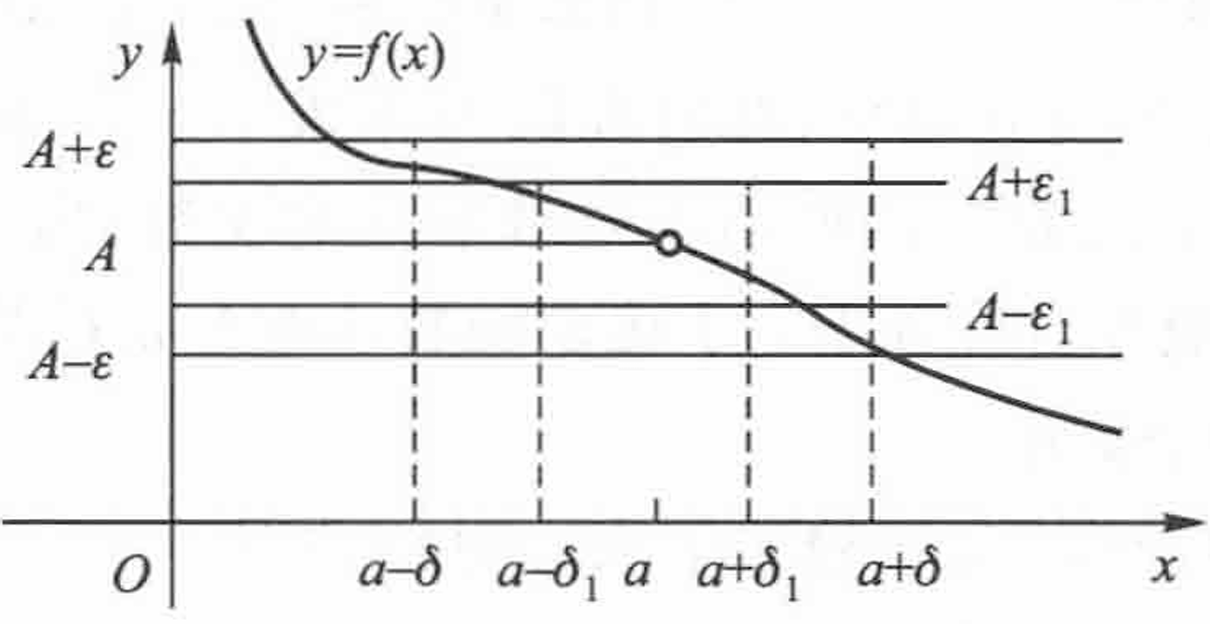
\includegraphics[width=0.7\linewidth]{eps-delta-graph.png}
    \end{figure}
\end{frame}

\begin{frame}{注意事项}
    \begin{itemize}
        \item 函数在某点的极限的$\varepsilon-\delta$定义中,定义域是$a$的\textbf{去心}邻域
        \item 因此,函数在$x=a$点是否有定义\textbf{不重要},此处函数值的情况可以是:
        \begin{itemize}
            \item 无定义或不存在
            \item 有定义(思考:函数值在此处有定义是否影响极限?)
        \end{itemize}
    \end{itemize}
\end{frame}

\begin{frame}{思考}
    考察函数
    \[
    f(x)=\left\{
    \begin{array}{ll}
        0, &x\ne0\\
        1, &x = 0
    \end{array}
    \right.
    \]
    在$0$处的极限$\displaystyle\lim_{x\rightarrow0}f(x)$
\end{frame}

\begin{frame}{讨论}
    当我们谈论函数在\textbf{某点}的极限时,我们讨论的范围是?
    \begin{itemize}
        \item 仅包含该点的去心邻域
        \item 函数在某处的极限,与该点的函数值无关
    \end{itemize}
\end{frame}

\begin{frame}{例(教材例2.25)}
    证明:
    \[
    \lim_{x\rightarrow 1}\frac{x^2-1}{3(x-1)}=\frac23
    \]
\end{frame}

\begin{frame}{Try it yourself! (23 Fall, ch.2 Quiz)}
    用$\varepsilon-\delta$语言证明:
    \[
    \lim_{x\rightarrow2}x^2=4
    \]
\end{frame}

\begin{frame}{放缩}
    \begin{itemize}
        \item 在使用定义证明极限值的时候,我们要尤其注意适时、适度的放缩.
        \item 使用如下方法:
        \begin{itemize}
            \item 某些函数的\textbf{有界性}
            \item 取部分上界,留下$|x-a|$项
        \end{itemize}
    \end{itemize}
\end{frame}

\begin{frame}{例}
    用极限的定义证明函数
    \[
    f(x)=\left\{
    \begin{array}{ll}
        -x^2-1,&x<0\\
        x^2+1,&x>0
    \end{array}
    \right.
    \]
    在$x=0$处的极限不存在.
\end{frame}

\begin{frame}{定理}
    $\displaystyle\lim_{x\rightarrow a}f(x)=A$的充分必要条件为
    \[
    f(a-0)=A\quad\text{ 且 }\quad f(a+0)=A
    \]
\end{frame}

\begin{frame}{例(课本 例2.36)}
    设函数
    \[
    f(x)=\left\{
        \begin{array}{ll}
            \sqrt x\sin\frac1x,&x>0,\\
            x^2+a,&x\le 0.
        \end{array}
    \right.
    \]
    求常数$a$,使得$f(x)$在$x\rightarrow0$时极限存在.
\end{frame}

\begin{frame}{海涅定理:数列与函数极限的联系}
    $\displaystyle\lim_{x\rightarrow a}f(x)=A$的充分必要条件为:对任一满足$\displaystyle\lim_{n\rightarrow\infty}x_n=a$且$x_n\ne a$
    的数列$\{x_n\}$均有\[
    \lim_{n\rightarrow\infty}f(x_n)=A.
    \]
    (推荐学有余力的同学尝试证明这个定理)
\end{frame}

\begin{frame}{例}
    求:
    \begin{align*}
        &(1)\qquad \lim_{x\rightarrow0}\sin\frac1x\\
        &(2)\qquad \lim_{x\rightarrow0}x\sin\frac1x
    \end{align*}
\end{frame}

\begin{frame}{极限的性质}
    \begin{itemize}
        \item 唯一性
        \item (局部)有界性
        \item (局部)保序性 $\Rightarrow$ (局部)保号性
        \item 夹逼定理
        \item \textbf{复合函数极限运算定理}
    \end{itemize}
\end{frame}

\begin{frame}{复合函数极限运算定理}
    若$\displaystyle \lim_{u\rightarrow b}f(u)=A,\lim_{x\rightarrow a}\varphi(x)=b,$且当$x\in\dot{U}(a)$时,$\color{red}\varphi(x)\ne b$,则
    \[
    \lim_{x\rightarrow a}f[\varphi(x)]=A.
    \]
    意味着我们可以进行如下调换
    \[
    \lim_{x\rightarrow a}f[\varphi(x)]\xlongequal{u=\varphi(x)}\lim_{u\rightarrow b}f(u)=A.
    \]
    思考:为什么一定要求$\varphi(x)\ne b$?
\end{frame}

\begin{frame}{思考}
    函数$f(x),g(x)$满足
    \[
    f(x)=\left\{
    \begin{array}{ll}
        0, &x\ne0\\
        1, &x = 0
    \end{array}
    \right.,\quad g(x)=0
    \]
    求$\displaystyle\lim_{x\rightarrow0}f(g(x))$
\end{frame}

\section{重要函数极限}

\begin{frame}{$\displaystyle\lim_{x\rightarrow0}\frac{\sin x}{x}=1$}
    课本P75:
    \begin{figure}
        \centering
        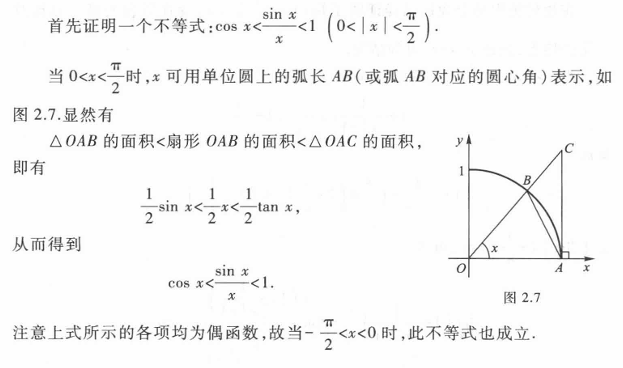
\includegraphics[width=0.7\linewidth]{sinxx.png}
    \end{figure}
    此方法涉及循环论证(将在第三章讲到)
\end{frame}

\begin{frame}{例}
    求
    \[
    \lim_{n\rightarrow\infty}n\sqrt{n}\Big(\tan(\frac{x}{\sqrt n})-\sin(\frac{x}{\sqrt n})\Big)
    \]
\end{frame}

\begin{frame}{$e$}
    与数列极限中$e$的定义类似:
    \[
    \lim_{x\rightarrow\infty}(1+\frac1x)^x=e
    \]
    进行$t=1/x$代换:
    \[
    \lim_{t\rightarrow0}(1+t)^{\frac1t}=e
    \]
    \color{red}注意:
    \[
    \lim_{t\rightarrow0}(1+\frac{1}{t})^t=1
    \]
\end{frame}

\begin{frame}{例}
    求
    \[
    \lim_{x\rightarrow a}\left(\frac{\sin x}{\sin a}\right)^{\frac{1}{x-a}}
    \]
\end{frame}

\section{无穷小}

\begin{frame}{定义}
    若$x\rightarrow a$时,$f(x)\rightarrow 0, g(x)\rightarrow 0$,考虑$\displaystyle\lim_{x\rightarrow a}\frac{f(x)}{g(x)}=l\in\mathbb R$:
    \begin{itemize}
        \item $l=0\Leftrightarrow$\\$x\rightarrow a\text{ 时,} f(x)$是比$g(x)$高阶的无穷小,记作$f(x)=o(g(x))$
        \item $l\ne0\Leftrightarrow$\\$x\rightarrow a\text{ 时,} f(x)$是与$g(x)$同阶的无穷小,记作$f(x)=O(g(x))$.\\
        若$l=1$则称$x\rightarrow a\text{ 时,}f(x)$与$g(x)$是等价无穷小,$f(x)\sim g(x)$.
    \end{itemize}
\end{frame}

\begin{frame}{定义}
    若$\displaystyle\lim_{x\rightarrow a}f(x)=0,$且存在常数$c\ne0,k>0,$使得
    \[
    \lim_{x\rightarrow a}\frac{f(x)}{(x-a)^k}=c,
    \]
    则称$x\rightarrow a$时,$f(x)$是\textbf{标准无穷小}$x-a$的$k$阶无穷小,简称$f(x)$是$k$阶无穷小,$c(x-a)^k$是$f(x)$的主部
\end{frame}

\begin{frame}{使用方法}
    \begin{itemize}
        \item 乘除:等价无穷小可以替换
        \item 加减:等价无穷小\textbf{有条件地}替换
    \end{itemize}
\end{frame}

\begin{frame}{简例}
    $f(x)=x+2x^2,g(x)=x-3x^2$,计算
    \[
    \lim_{x\rightarrow 0}\frac{f(x)-g(x)}{x^2}
    \]
\end{frame}

\begin{frame}{注意事项}
    \begin{itemize}
        \item 乘除运算不会导致无穷小的主部消失;
        \item 加减运算可能会导致无穷小主部恰好抵消,则此时剩余的更高阶无穷小\textbf{不可忽略}.
    \end{itemize}
\end{frame}

\begin{frame}{例 (24Fall Midterm 7.)}
    设$\displaystyle\lim_{x\rightarrow0}\frac{\cos x - 1 + f(x)}{x^3}=1$,求$\displaystyle\lim_{x\rightarrow0}\frac{f(x)}{\sin^2x}$
\end{frame}


% -------------------------------------------------------
% \section*{}
% \begin{frame}
% \vspace{25pt}
% \[
% \text{\Huge Office Hour}
% \]
% \end{frame}

\end{document}